% investigation and optimisation of 
%	possible trigger optimisation
%	b-tagging (pile-up, boost/sub-jets, new layer(timely)), jet-charge, PUPPI
%	top-tagging (sub-jets, kinematic reconstruction, MVA/Matrix-Element etc.)
% measurement of cross section and evaluation of systematic uncertainties
%timetable
%\noindent\textit{1. Trigger-chain selection and optimisation; $t\bar{t}t\bar{t}$ process baseline selection. (low-risk)}\\
%To select candidate \fourtop events on-line, different existing CMS trigger paths will be used depending on the decay channel in focus. Thus, for example, dedicated single-muon and single-electron triggers can be utilised for $l$+jets channel, while the $ll$+jets selection can take the advantage of existing di-lepton triggers. Presence of a $b$-jet can be possibly included to the High-Level trigger requirements also. For the all-hadronic \fourtop channel no dedicated triggers exist, however, the applicability of CMS multi-jet and high-$\hight$ trigger chains developed for SUSY analyses can be explored, otherwise a\textbf{ dedicated trigger path will be designed} for the 2017--2018 running phase. In case such a trigger configuration will be developed, one can benefit from tunning the trigger specifically to have high acceptance for \fourtop events, for example $p_T$ thresholds can be lowered while maintaining acceptable trigger rates. Well established techniques will be used to measure efficiencies and corresponding systematic uncertainties attributed to those triggers. I have \textbf{experience in both development and optimising new trigger} configuration as well as the measurements of existing trigger performance. Therefore this task is considered as having a \textbf{low risk} and is a natural starting point for further deployment of the analysis.
%\newline
%
%\noindent\textit{2. $b$-tagging performance optimisation. (medium-risk)}\\
%After selecting suitable trigger chains and ensuring appropriate quality of selected final-state leptons and jets using off-line selection criteria, further restrictions on $b$- and light-flavour-jet multiplicity will be imposed to reduce the background from top-pair production associated with multiple jets. Any particular choice is always a trade-off between selection efficiency and purity of the data sample, and thus is subject to optimisation.

After imposing appropriate selection criteria on $b$-quark multiplicity, the remaining dominant background contribution will be due to \ttbb, for zero-leptons or single- and two-leptons channels, respectively. The production cross sections of \ttbb process is approximately two orders of magnitude larger~\cite{Bevilacqua:2014qfa} than that of \fourtop. For this reason, the next logical step would be to identify and reconstruct (additional) top decays.
%\newline

\noindent\textit{1. Direct searches for BSM processes and SM $t\bar{t}t\bar{t}$ production measurement in single-lepton and dilepton channels. (medium-risk)}\\

A search for and first observation of SM $t\bar{t}t\bar{t}$ production in the single-lepton channel is the first goal of this proposal. 
Whenever the data sample is fixed and backgrounds are reasonably understood, the measurement of signal cross section is a well-established process. For the low-level calibrations such as (in)efficiencies and scale factors necessary to get agreement between data and simulation, the intention is to rely on the software framework used in the VUB group, which is shared between many CMS analyses in top physics and includes all necessary corrections. However, it will be necessary to make sure that the estimation of trigger efficiencies, calibrations and determination of scale factors is sufficient before this effort can start.

Given the first indications of an excess observed in 2016 dataset, the immediate target of the first WP is to establish or exclude the signal using the 2017 and 2018 LHC datasets.  
Before claiming an observation, careful scrutiny of various backgrounds is needed, including detailed study of Monte Carlo modelling of $t\bar{t}+X$ backgrounds and checking potential contributions from sources with fake leptons, such as events with hadronic jets misidentified as muons or electrons, etc. 

Decay of four top quarks in the single-lepton mode results in ten jets in the final state. Matrix-element predictions of such high jet multiplicity $t\bar{t}$ events are not possible with existing event generators, therefore, background modelling in this corner of phase space relies on parton shower models that typically have several free parameters fitted to the data. Comparison of $t\bar{t}+X$ predictions based on different parton shower models is one step towards better understanding of the observed excess. Alternatively, data-driven estimate of the $t\bar{t}$ cross section in high jet multiplicity events can be obtained from extrapolation from better understood low multiplicity regions assuming so-called "staircase"~\cite{Ellis:1985vn} and "Poisson"~\cite{Gerwick:2012hq} scaling predicted by QCD. Similar technique was applied in ATLAS~\cite{Aaboud:2017faq}.

To measure the $t\bar{t}t\bar{t}$ signal, a fit to multivariate discriminator distribution (obtained with machine learning) will be performed in order to estimate the amount of \fourtop events in the data. A simultaneous fit to different background- (signal-) enhanced event categories will be performed to constrain the background and determine the number of signal events. I have a good knowledge of various fitting approaches, including multidimensional likelihood fits to the distributions with low counting statistics to effectively work on this task.

The experimental and theoretical sources of systematic uncertainty for such a method have to be taken into account as both can affect the shape and normalisation of the measured distributions. These uncertainties will be included as nuisance parameters into the above-mentioned likelihood fits.
%Examples of theoretical uncertainty include the ones due to the variation of renormalisation and factorisation scales in perturbative calculations or the variation of the matching scale in the parton-shower-matching procedure. The experimental uncertainties arise, for example, due to finite accuracy of jet energy calibration, b- and top-identification procedures, luminosity etc. 
The most important systematic uncertainties in a \fourtop analysis are from the simulation of $t\bar{t}$ production, and the b-identification. For the former I have unique experience due to my role as MC contact, and the latter the experts are present at the VUB. 

Assuming the currently known SM cross section for $t\bar{t}t\bar{t}$ production, the complete LHC Run 2 dataset collected in 2018 should be sufficient to make a statistically significant observation of $t\bar{t}t\bar{t}$ SM production, which would be an important result from CMS. However, considering the first results outlined in the previous sections, there are hints that $t\bar{t}t\bar{t}$ could be observed earlier, which is what WP2 focuses on. 

The analysis of single-lepton events can be performed in parallel with a PhD student from University of California Riverside who focuses on the opposite-sign dilepton final state and who I am currently co-supervising. 
%Individual channels will differ in the details of systematic studies, mainly because of the variations in the background strength and sources composition. 

The ongoing effort is an extension of the previous results obtained using 2015 dataset~\cite{Sirunyan:2017tep}. First results with 2016 data, outlined in the previous sections, \textbf{demonstrate feasibility} of this WP. Moreover, a backup scenario for background estimation is envisaged. \textbf{My experience in ongoing and previous projects makes me an ideal candidate to carry out described tasks.}
The success in WP1 partially depends on external input, however the analysis is based on well-established tools and follows standard strategy adopted in the field. Taking these conditions into account, this WP is considered as \textbf{medium-risk.} \textbf{An observation of the $t\bar{t}t\bar{t}$ process will have significant impact on the field as the first observation of a BSM-sensitive SM \tttt process is  novel enough to be published in a high-impact peer-reviewed journal.}


%\newline


\noindent\textit{2. Top-tagging performance optimisation and searches for $t\bar{t}t\bar{t}$ in all-hadronic channel. (high-risk)}\\
\textcolor{\mynew}{
The standard model four top production is characterised by moderate transverse momentum of produced tops, therefore decay products can be resolved in the detector. At $\sqrt{s}$=14 TeV, however, a significant fraction of top quarks is expected to be produced with large Lorentz-boost, leading to strongly collimated decay products which end-up in a single jet. 
Moreover, as was mentioned, many BSM models predict heavy states, resulting in a large boost of the decay products. Thus the searches for such states in resolved topology events, as in WP1, are less efficient and reconstruction of boosted top decays becomes crucial for direct searches. 
}
\textcolor{\mynew}{
The top-tagging is currently an active area of research and many novel techniques were proposed over the last years. In particular, the HepTopTagger algorithm~\cite{heptoptagger} demonstrated very good performance in the recent search for pair production of vector-like T quarks in events with similar event signature in CMS~\cite{Khachatryan:2015oba}. Besides that, the CMSTopTagger~\cite{Kaplan:2008ie} employs a different jet deconstruction approach which is more suitable for highly boosted top decays. More algorithms exist including shower-deconstruction tagger and N-subjettiness algorithm, the applicability of which~\cite{CMS:2014fya} still has to be explored. Therefore, in order to enhance sensitivity to BSM \fourtop signal, especially in the zero-leptons decay channel, the investigation of different techniques is foreseen in this project. To my knowledge, besides the discontinued attempt of $W$-tagging at UGent, this can be the \textbf{first significant effort on jet substructure in Belgium}.
}
\textcolor{\mynew}{
This task goes hand-in-hand with optimisation of the $b$-tagging in sub-jet environment. A better performance of the $b$-tagging can give a significant gain in terms of light-flavour background rejection, therefore I plan to investigate novel tools designed in CMS~\cite{Bertolini:2014bba} and explore new promising jet-charge identification technique developed recently in ATLAS~\cite{Aad:2015cua,ATLAS:2015jetcharge}.
}
\textcolor{\mynew}{
This WP is exploratory in nature and assessed as a \textbf{high-risk and high-impact}. This effort is very timely with the LHC instantaneous luminosity increase foreseen for the year 2018 and may have a positive impact for other studies in the collaboration, for example, for 'high-profile' $ttH \rightarrow ttb\bar{b}$ search planned to be performed by the hosting group. The all-hadronic channel may require more significant effort investment. There are diverse challenges inherent to severe not completely understood QCD background. In addition, input from CMS collaborators on performance of b-tagging algorithms in boosted regime is needed. Eventually, the success in this project relies on novel tools. Nevertheless, I believe, I am a perfect candidate for this pioneering effort, since I have a wide knowledge acquired during my doctoral studies in the area of track reconstruction and broad experience in jet and top analyses.
}
\textcolor{\mynew}{
Without doubt, the discovery of a new state will have major impact on the field, but negative result is also worth an effort since very little is known about this extreme corner of phase space. The obtained results will be \textbf{published in a refereed journal}. As previously mentioned, the development of substructure algorithms is of great interest in the field. Therefore, it is expected that new developments will be included in a \textbf{performance paper} by the CMS collaboration.
}
%A more general approach to top tagging, applicable in both boosted and un-boosted topologies, is the Matrix-Element (ME) method. In the ME method, a statistical classifier based on final-state kinematic information and LO matrix elements is constructed to test how likely is that given event originates from signal or background source. This technique was recently demonstrated in $ttH \rightarrow ttbb$ analysis~\cite{MartixElementMethod} and proved to be very effective. In addition to that, the approach can be generalised to decide, for example, whether a given combination of jets and leptons arise from the common top decay. Nevertheless, using theoretical input in the selection procedure, unavoidably introduces model dependence in the measurements. Therefore I propose a possibly novel approach in which this problem can be facilitated by combining ME method with MVA techniques. I propose instead of using weights (which are typically available at LO only) directly in the statistical classifier, to utilise them for seeding multivariate regression model to derive improved weights using available higher-order calculations and/or data.

%The studies for single- and two-leptons channels will largely benefit from the experience developed by the host institute, while in the zero-leptons channel my expertise in QCD jet analysis will be a valuable complement.%As described above, the reconstruction of \fourtop final-state suffers from combinatorial ambiguity in assigning the decay products to theirs parent $t$-quarks. This feature helps to mitigate combinatorial problem, because it suggests natural candidates for decay products originating from the same parton. 

%In the single-lepton channel one can benefit from the constrained kinematics of the event. If the lepton is well isolated and its momentum is reliably measured, the four-momentum of the neutrino from the $W$ decay can be reconstructed as well. Considering a single $t\bar{t}$ pair, four equations: momentum conservation, two constraints due to the $W^\pm$ mass and equality of $t$ and $\bar{t}$ masses, can be used to determine four unknown components of the neutrino momentum vector. This information will help to improve the resolution of the various quantities derived from the momenta of final-state objects. In principle, same technique can be applied in the zero-lepton channel as well, although due to much worse precision of the jet measurement and even larger combinatorial ambiguity, the solution of the constrain equations can be less robust.
%\newline


\noindent\textit{3. Results combination and interpretation. (low/medium-risk)}\\
\textcolor{\mynew}{
The aim of this WP is to perform statistical combination the results obtained in different channels and interpret searches performed in WP1 and WP2 using phenomenological models. As was shown by the applicant in~\cite{Sirunyan:2017tep}, combination of SM \tttt searches in different channels can substantially improve the sensitivity of the search, due to complementarity of information provided by different channels. Although, the improvement in the referenced publication, is attributed mainly to increase of the signal efficiency due to summing contributions from different decay modes, the synergy of independent channels will become more prominent, when statistical component of the uncertainty can be reduced using larger datasets accumulated in 2016--2018. For example, rates of rare backgrounds, such as $t\bar{t}Z$ and $t\bar{t}W$, contributing in both single-lepton and dilepton channels can be better constrained in dedicated control regions of dilepton analysis and applied in single-lepton search. On the other hand, dilepton analysis can profit from larger branching fraction of $t\bar{t} \rightarrow l+\mathrm{jets}$ to better constrain jet multiplicity spectrum, the modelling of which was among dominant sources systematic uncertainty, so far. Combination will be performed using statistics tools, that are widely used in ATLAS and CMS experiments. The applicant has all necessary skills to effectively accomplish this task.
}
\textcolor{\mynew}{
A novel goal of this WP is a bottom-up interpretation of the results of the searches using four top EFT model~\cite{DegrandeEFTthesis}. In case, when no BSM states will be observed, the limits on coupling of effective operators will provide constraints on potential physics scenario beyond the standard model. In contrast to phenomenological interpretation using specific BSM models, such as e.g.~\cite{Sirunyan:2017uyt}, where very restrictive assumptions on model parameters had to be made ($\tan \beta=$1\footnote{In this analysis, the so-called 2HDM model was considered, where $\tan \beta$ is a ratio of vacuum expectation values of $H_u$ and $H_v$ fields.}), EFT analysis helps to draw more universal conclusions about potential new physics. Thus, such results will extend the scope and impact of existing interpretations of four top production data. 
}
\textcolor{\mynew}{
An initial attempt of EFT interpretation of 2015 results, described above, \textbf{demonstrates the potential of new data and my capability to successfully perform this sub-project}. The outlined analysis, is limited by assumption that detector acceptance of \tttt final state resulting from effective interaction of top quarks is the same as for SM \tttt production, which is not the case if the EFT cut-off scale is high, as mentioned in WP2. In order avoid potential ambiguities, the impact on experimental sensitivity of  differences in two production mechanisms will be taken into account in detailed CMS simulations of EFT processes. There are only 5 dim-6 four-fermion operators contributing to production of four top quarks in proton-proton collisions. However, model parameters scan quickly becomes a formidable task, as soon as full detector simulations are employed. Nevertheless, polynomial dependence of EFT predictions on model parameters allows to interpolate calculations using only a small set reference computation, thus, making this goal achievable. \textbf{My experience with the MC generation in CMS PdmV group is relevant to ensure timely production of necessary MC simulations.} This analysis will complement ongoing studies in UGent, where other rare $t\bar{t}W$ and $t\bar{t}Z$ processes are analysed within EFT framework. All these studies fit nicely with more ambitious effort of SM EFT analysis of all existing $t\bar{t}$ data, which is also carried out at VUB and XXX. 
}
\textcolor{\mynew}{
The two sub-projects detailed in this WP are assessed as low and medium risk, respectively. The first sub-project is a new incarnation of the previous studies, extended to all-hadronic channel. While the second sub-project is more innovative, but is build on my expertise developed in the past year. The work on these projects can be started as soon as first results with new data appear. The outcome of these all will be published \textbf{together with the experimental results} outlined above or in a \textbf{separate publication}.
}
%The modified frequentist $\mathrm{CL_s}$ approach~\cite{Junk:1999kv,Read:2002hq} can be used to assess the statistical significance of the signal in case of observation or to establish the limits on the mass and production cross section, as well as to combine results obtained in different channels. \textbf{This WP will build on the expertise of other researchers in the institution and strong collaboration with the authors of respective theoretical predictions and thus has potential risks.}  A bottom-up approach would be the interpretation of the data using the EFT calculations. together with cooperation with the phenomenology groups in Brussels is the perfect fit to complete this task in an effective manner.
%
%\begin{itemize}
%\item EFT
%\begin{itemize}
%\item dim-6 four fermion
%\item limitation of Bsc analysis is the assumption of similarity of acceptance for EFT and SM 
%\item proof of feasibility 
%\item analytic parametrisation
%\item full or fast mc simulations
%\end{itemize}
%\item +Combination of sl, dl and all hadronic
%\item +higgs combine tool
%\item +experience in combination of 2015
%\end{itemize}
%

%\newline

The Gantt chart (allocated time interval and estimated risk) for the envisaged WPs and corresponding subtasks is illustrated in Figure~\ref{fig:gantt_new}. The publication procedures are not included into the chart because of the specific nature of the publication policy in the CMS collaboration. In general, the foreseen journal articles will be prepared in parallel to the outlined active stages of research. The estimated effort includes service work to qualify as a CMS author, which amounts to 3 month/year.
%\begin{sidewaysfigure}[p!]
     \begin{ganttchart}[%Specs
             y unit title=0.5cm,
             y unit chart=0.5cm,
             vgrid,hgrid,
             title height=1,
             title label font=\bfseries\footnotesize,
             bar/.style={fill=blue},
             bar height=0.7,
             group right shift=0,
             group top shift=0.7,
             group height=.1,
             group peaks width={0.2},
             inline]{1}{36}
            %labels
            \ganttset{group/.append style={orange},
            milestone/.append style={red},
            progress label node anchor/.append style={text=red}}
            \ganttset{progress label text={}, link/.style={black, -to}}
            \gantttitle{BSM searches in events with four top quark signature at $\sqrt{s}=13/14$ TeV at the LHC}{36}\\  % title 1
            \gantttitle[]{2017}{3}                 % title 2
            \gantttitle[]{2018}{12}
            \gantttitle[]{2019}{12}
            \gantttitle[]{2020}{9}  \\              
            \gantttitle{Q4}{3}                      % title 3
            \gantttitle{Q1}{3}
            \gantttitle{Q2}{3}
            \gantttitle{Q3}{3}
            \gantttitle{Q4}{3}
            \gantttitle{Q1}{3}
            \gantttitle{Q2}{3}
            \gantttitle{Q3}{3}
            \gantttitle{Q4}{3}
            \gantttitle{Q1}{3}
            \gantttitle{Q2}{3}
            \gantttitle{Q3}{3}\\
            \ganttnewline
            % WP1
            \ganttgroup[group/.append style={fill=blue}]{\hspace{1ex}Event selection (WP1)}{1}{6}\\
            \ganttbar[progress=100,inline=false,bar/.append style={fill=green}]{\parbox[c][1ex][c]{0.12\textwidth}{Trigger chain} }{1}{6}\\
%            \ganttbar[progress=100,inline=false,bar/.append style={fill=orange}]{\parbox[c][1ex][c]{0.12\textwidth}{$b$-tagging}}{1}{15}\\
			\ganttnewline
        	% WP2
        	\ganttgroup[group/.append style={fill=blue}]{Measurement of the SM \fourtop cross section (WP2)}{3}{18} \\
        	\ganttbar[progress=100,inline=false,bar/.append style={fill=green}]{$l$+jets channel}{3}{13} \\
        	\ganttbar[progress=100,inline=false,bar/.append style={fill=green},name=ljetsm]{$ll$+jets channel}{7}{18} \\
        	\ganttbar[progress=100,inline=false,bar/.append style={fill=orange},name=alljetsm]{all jets channel}{9}{18} \\   
        	\ganttnewline
        	% WP3
        	\ganttgroup[group/.append style={fill=blue}]{\hspace{1ex}Event reconstruction and top tagging (WP3)}{12}{23}\\
        	\ganttbar[progress=100,inline=false,bar/.append style={fill=orange}]{\parbox[c][1ex][c]{0.12\textwidth}{top-tagging}}{12}{23}\\
        	\ganttnewline
            % WP4
			\ganttgroup[group/.append style={fill=blue}]{Direct BSM searches (WP4)}{12}{30} \\
            \ganttbar[progress=100,inline=false,bar/.append style={fill=red}]{$l$+jets channel}{12}{23} \\
            \ganttbar[progress=100,inline=false,bar/.append style={fill=red},name=ljets]{$ll$+jets channel}{16}{27} \\
            \ganttbar[progress=100,inline=false,bar/.append style={fill=red},name=alljets]{all jets channel}{20}{30}  \\   
            \ganttnewline
        	% WP5
            \ganttgroup[group/.append style={fill=blue}]{Combination and interpretation (WP5)}{23}{36} \\
%            \ganttbar[progress=100,inline=false,bar/.append style={fill=green},name=comb1]{}{15}{18}
            \ganttbar[progress=100,inline=false,bar/.append style={fill=green},name=comb2]{%
            \parbox[c][1ex][c]{0.14\textwidth}{Results combination}}{23}{29} \\
%   	        \ganttlink[link mid=.159]{alljets}{comb}
%            \ganttlink[link mid=.4]{ljets}{comb}
%			\ganttbar[progress=100,inline=false,bar/.append style={fill=green}]{}{17}{20}
            \ganttbar[progress=100,inline=false,bar/.append style={fill=green}]{%
            \parbox[c][1ex][c]{0.14\textwidth}{SMF Interpretation}}{26}{36} \\
%            \ganttbar[progress=100,inline=false,bar/.append style={fill=orange}]{}{17}{20}
            \ganttbar[progress=100,inline=false,bar/.append style={fill=orange}]{\parbox[c][1ex][c]{0.14\textwidth}{EFTF Interpretation}}{26}{36}
              
              % Legend
%              \draw [fill=white] (10.7,-1.7) rectangle (16.5,-3.9);
              \draw [fill=white] (10.7,-1.7) rectangle (16.5,-3.8);
              \node [fill=white,anchor=west] at (12.7,-2.15) {Low risk};
              \draw [fill=green] (11.1,-2.1) rectangle (12.5,-2.3);
              \node [fill=white,anchor=west] at (12.7,-2.75) {Medium risk};
              \draw [fill=orange] (11.1,-2.7) rectangle (12.5,-2.9);
              \node [fill=white,anchor=west] at (12.7,-3.45) {High risk};
              \draw [fill=red] (11.1,-3.3) rectangle (12.5,-3.5);
        \end{ganttchart}
        \caption{Time-line of the proposed project. Each year of the fellowship mandate is divided into intervals of three months (Q1-4). The extend of the color bands indicates the start and the end of corresponding task, while their color encodes the risk estimate. In this figure, SMF --- simplified model framework; EFTF --- effective field theory framework.}
        \label{fig:gantt}
\end{sidewaysfigure}
\begin{figure}[h!]
\centering
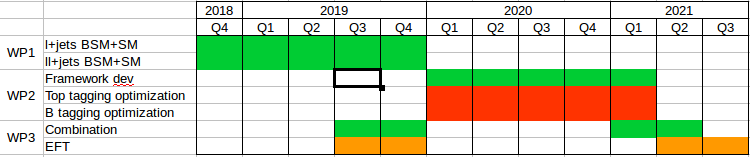
\includegraphics[width=\linewidth]{figures/gantt_new}
        \caption{Time-line of the proposed project. Each year of the fellowship mandate is divided into intervals of three months (Q1-4). The extend of the color bands indicates the start and the end of corresponding task, while their colour encodes the risk estimate (Green---low risk, Orange---medium risk, Red---high-risk). In this figure, EFT --- effective field theory.}
\label{fig:gantt_new}
\end{figure}
